\documentclass[12pt]{article}

\usepackage[margin=1in]{geometry}
\usepackage{amsmath,amssymb}
\usepackage{graphicx}
\usepackage{booktabs}
\usepackage{natbib}
\usepackage{setspace}
\usepackage{hyperref}
\usepackage{caption}
\usepackage{subcaption}
\usepackage{float}
\usepackage{pdflscape}
\usepackage[T1]{fontenc}
\usepackage{lmodern}
\usepackage{catchfile}
\newcommand{\inputifexists}[1]{\IfFileExists{#1}{\input{#1}}{\textit{[Table not yet generated.]}}}

\bibliographystyle{aer}

\onehalfspacing

\title{Urban Air Pollution and Time Losses: \\
Evidence from Cyclists in London --- Revisited}

\author{Joris Klingen \and Jos van Ommeren}

\date{\today}

\begin{document}

\maketitle

\begin{abstract}
We replicate and extend \citet{klingen2020urban}, who found that a 10~ppb increase in ozone reduces cycling speed by 0.3--0.4\% using 42 million London bike-share trips (2013--2017). Extending the sample to 108 million trips through 2025, we confirm a negative ozone--speed relationship across all four identification strategies. Point estimates in the extended and post-2017 samples are at least as large as in the original period, indicating that the effect has not diminished despite substantial changes in London's air quality and cycling landscape.

\medskip
\noindent \textit{Keywords}: air pollution, ozone, physical effort, cycling, productivity, replication \\
\noindent \textit{JEL Codes}: I18, J24, Q53, R41
\end{abstract}

\newpage

%% ============================================================
\section{Introduction} \label{sec:intro}
%% ============================================================

\citet{klingen2020urban} provided novel evidence that ambient ozone reduces cycling speed, using 42 million Santander Cycles trips during 2013--2017. Their preferred within-day estimate implied that a 10~ppb increase in ozone reduces speed by about 0.4\%, with effects emerging at concentrations as low as 20~ppb---far below regulatory standards.

We revisit their analysis with two objectives. First, we replicate the original results on the 2013--2017 sample, implementing the same four identification strategies (within-day, between-day, spatio-temporal, cyclist panel) without traffic controls, which the original study showed to be inconsequential. Second, we extend the analysis to 2013--2025, tripling the sample to over 108 million trips. We also estimate models on the post-2017 subsample alone (2018--2025) to test whether the relationship holds in a period that includes COVID-19, the Ultra Low Emission Zone expansion, and substantial cycling infrastructure changes.

Our replication confirms the core findings. In the extended and post-2017 samples, the within-day ozone coefficient is roughly twice the replication estimate, suggesting the effect may be \emph{larger} in more recent data. The between-day and spatio-temporal strategies yield consistent negative coefficients. Robustness checks---non-linearity analysis, lag/lead tests, and median speed regressions---support the original conclusions.


%% ============================================================
\section{Methods and Data} \label{sec:methods}
%% ============================================================

We implement the four identification strategies of \citet{klingen2020urban}; see their paper for details. All models are estimated on weekdays only.

\paragraph{Within-day.} Hourly city-level speed is regressed on ozone (per 10~ppb), flexible weather controls (temperature dummies, pressure, humidity, rain, radiation dummies, wind, 8-hour temperature and rain lags), and co-pollutant controls (SO$_2$, NO$_x$ and PM$_{2.5}$ dummies), with day and day-of-week$\times$hour fixed effects. WLS with trip counts as weights; SEs clustered by date.

\paragraph{Between-day.} Daily aggregates with year-month and day-of-week fixed effects.

\paragraph{Spatio-temporal.} Zone-day aggregates (5 monitoring zones, 2~km radius; a trip is assigned to a zone if both its origin and destination station are within 2~km of the monitor), with day, zone, and zone-month (or zone-week) fixed effects and NO$_x$ dummies.

\paragraph{Cyclist panel.} Pseudo-cyclists identified from repeat commuters on the same route, hour, and month with departure-time regularity below the 5th percentile of the random uniform distribution ($\geq$4 trips). Cyclist fixed effects absorb route and time-of-day preferences.

\paragraph{Data.} Trip data are from Transport for London's Santander Cycles. Air quality data (O$_3$, NO$_2$, NO, PM$_{2.5}$, SO$_2$) are from the London Air Quality Network (5 stations). Weather data are from the Open-Meteo archive. The replication sample covers 2013--2017 ($\approx$42M trips), the extended sample 2013--2025 ($\approx$108M trips), and the post-2017 sample 2018--2025 ($\approx$66M trips).

Table~\ref{tab:desc} reports descriptive statistics. Mean ozone is higher in the post-2017 period (25.4 vs.\ 18.9~ppb) while NO$_x$ has declined substantially (21.9 vs.\ 44.7~ppb), consistent with ULEZ effects. Mean cycling speed is slightly higher in recent years (12.5 vs.\ 12.0~km/h).

\begin{table}[H]
\centering
\caption{Descriptive statistics (hourly, trip-weighted).}
\label{tab:desc}

\medskip
\small Panel A: Replication (2013--2017).

\begin{tabular}{lrrrr}
\toprule
Statistic & Mean & St Dev. & Min & Max \\
\midrule
Speed (km/h) & 11.99 & 1.67 & 5.85 & 17.75 \\
Distance (km) & 2.81 & 0.28 & 1.40 & 5.36 \\
Duration (sec) & 1105.50 & 322.89 & 443.33 & 10658.68 \\
Number of trips & 1808.32 & 1078.90 & 4.00 & 6893.00 \\
Ozone (O\textsubscript{3}, ppb) & 18.85 & 11.61 & 0.04 & 78.28 \\
Nitrogen oxides (NO\textsubscript{x}, ppb) & 44.72 & 35.97 & 1.38 & 509.24 \\
Particulate matter (PM\textsubscript{2.5}, $\mu$g/m\textsuperscript{3}) & 13.53 & 10.37 & -2.60 & 114.87 \\
Sulphur dioxide (SO\textsubscript{2}, ppb) & 1.10 & 1.03 & -0.29 & 92.72 \\
\bottomrule
\end{tabular}


\medskip
\small Panel B: Post-2017 (2018--2025).

\begin{tabular}{lrrrr}
\toprule
Statistic & Mean & St Dev. & Min & Max \\
\midrule
Speed (km/h) & 12.47 & 1.65 & 1.24 & 22.72 \\
Distance (km) & 3.06 & 0.33 & 0.96 & 11.56 \\
Duration (sec) & 1118.56 & 299.65 & 247.42 & 24468.88 \\
Number of trips & 1863.05 & 1057.37 & 1.00 & 6642.00 \\
Ozone (O\textsubscript{3}, ppb) & 25.43 & 12.64 & 0.07 & 99.77 \\
Nitrogen oxides (NO\textsubscript{x}, ppb) & 21.94 & 19.44 & 0.28 & 270.19 \\
Particulate matter (PM\textsubscript{2.5}, $\mu$g/m\textsuperscript{3}) & 8.96 & 7.28 & -2.65 & 151.62 \\
Sulphur dioxide (SO\textsubscript{2}, ppb) & 0.59 & 0.64 & -0.69 & 52.24 \\
\bottomrule
\end{tabular}


\medskip
\footnotesize Means and standard deviations weighted by number of trips per hour.
\end{table}


%% ============================================================
\section{Results} \label{sec:results}
%% ============================================================

\subsection{Within-day estimation}

Table~\ref{tab:within} presents the within-day results. In the replication sample, a 10~ppb increase in ozone reduces speed by 0.052~km/h (column~1), closely matching the original estimate of $-0.053$. The effect nearly doubles in both the full extended sample ($-0.095$, column~2) and the post-2017 subsample ($-0.098$, column~3), all significant at the 1\% level.

The sorting tests show no meaningful effect of ozone on trip distance (columns~4--6) or log trips (columns~7--9), confirming that the speed effect reflects physiological impairment rather than compositional changes.

\begin{table}[H]
\centering
\caption{Within-day estimation.}
\label{tab:within}
\begingroup
\centering
\begin{tabular}{lccccccccc}
   \tabularnewline \midrule \midrule
   Dependent Variables: & \multicolumn{3}{c}{mean\_speed} & \multicolumn{3}{c}{mean\_dist} & \multicolumn{3}{c}{log(n\_trips)}\\
                         & Speed (R)       & Speed (E)       & Speed (P)       & Dist (R) & Dist (E)        & Dist (P)        & Trips (R) & Trips (E)      & Trips (P) \\   
   Model:                & (1)             & (2)             & (3)             & (4)      & (5)             & (6)             & (7)       & (8)            & (9)\\  
   \midrule
   \emph{Variables}\\
   O3\_10                & -0.0723$^{***}$ & -0.0813$^{***}$ & -0.0724$^{***}$ & 0.0015   & -0.0134$^{***}$ & -0.0149$^{***}$ & -0.0002   & 0.0042$^{***}$ & 0.0042$^{***}$\\   
                         & (0.0155)        & (0.0101)        & (0.0119)        & (0.0036) & (0.0025)        & (0.0030)        & (0.0012)  & (0.0008)       & (0.0009)\\   
   \midrule
   \emph{Fixed-effects}\\
   date                  & Yes             & Yes             & Yes             & Yes      & Yes             & Yes             & Yes       & Yes            & Yes\\  
   dow\_hour\_daylight   & Yes             & Yes             & Yes             & Yes      & Yes             & Yes             & Yes       & Yes            & Yes\\  
   \midrule
   \emph{Fit statistics}\\
   Observations          & 28,692          & 76,454          & 47,762          & 28,692   & 76,454          & 47,762          & 28,692    & 76,454         & 47,762\\  
   R$^2$                 & 0.92495         & 0.92579         & 0.93478         & 0.91823  & 0.92239         & 0.92643         & 0.99840   & 0.99795        & 0.99811\\  
   Within R$^2$          & 0.22063         & 0.18500         & 0.21027         & 0.23430  & 0.18739         & 0.24371         & 0.98354   & 0.97869        & 0.97774\\  
   \midrule \midrule
   \multicolumn{10}{l}{\emph{Clustered (date) standard-errors in parentheses}}\\
   \multicolumn{10}{l}{\emph{Signif. Codes: ***: 0.01, **: 0.05, *: 0.1}}\\
\end{tabular}
\par\endgroup


\medskip
\footnotesize WLS with trip counts as weights. SEs clustered by date. (R) = 2013--2017, (E) = 2013--2025, (P) = 2018--2025.
\end{table}


\subsection{Between-day estimation}

Table~\ref{tab:between} reports between-day results. The replication coefficient ($-0.286$, column~1) is larger than the within-day estimate, consistent with the original study and with the fact that between-day variation in ozone may capture additional cumulative exposure effects. The post-2017 estimate ($-0.084$, column~3) is smaller but remains significant at the 1\% level. The distance and trip-count coefficients are small and mostly insignificant.

\begin{table}[H]
\centering
\caption{Between-day estimation.}
\label{tab:between}
\begingroup
\centering
\begin{tabular}{lccccccccc}
   \tabularnewline \midrule \midrule
   Dependent Variables: & \multicolumn{3}{c}{mean\_speed} & \multicolumn{3}{c}{mean\_dist} & \multicolumn{3}{c}{log(n\_trips)}\\
                & Speed (R)       & Speed (E)       & Speed (P)      & Dist (R)     & Dist (E) & Dist (P) & Trips (R)     & Trips (E) & Trips (P) \\   
   Model:       & (1)             & (2)             & (3)            & (4)          & (5)      & (6)      & (7)           & (8)       & (9)\\  
   \midrule
   \emph{Variables}\\
   O3\_10       & -0.2759$^{***}$ & -0.1170$^{***}$ & -0.0770$^{**}$ & 0.0122$^{*}$ & 0.0038   & 0.0003   & -0.0034$^{*}$ & -0.0010   & $-3.64\times 10^{-5}$\\    
                & (0.0575)        & (0.0278)        & (0.0325)       & (0.0067)     & (0.0034) & (0.0041) & (0.0020)      & (0.0010)  & (0.0012)\\   
   \midrule
   \emph{Fixed-effects}\\
   yearmonth    & Yes             & Yes             & Yes            & Yes          & Yes      & Yes      & Yes           & Yes       & Yes\\  
   dow          & Yes             & Yes             & Yes            & Yes          & Yes      & Yes      & Yes           & Yes       & Yes\\  
   \midrule
   \emph{Fit statistics}\\
   Observations & 1,202           & 3,244           & 2,042          & 1,202        & 3,244    & 2,042    & 1,202         & 3,244     & 2,042\\  
   R$^2$        & 0.54039         & 0.68191         & 0.73560        & 0.82163      & 0.90513  & 0.87642  & 0.99580       & 0.99531   & 0.99531\\  
   Within R$^2$ & 0.29909         & 0.20799         & 0.23017        & 0.56121      & 0.47393  & 0.45371  & 0.98832       & 0.98754   & 0.98800\\  
   \midrule \midrule
   \multicolumn{10}{l}{\emph{Clustered (date) standard-errors in parentheses}}\\
   \multicolumn{10}{l}{\emph{Signif. Codes: ***: 0.01, **: 0.05, *: 0.1}}\\
\end{tabular}
\par\endgroup


\medskip
\footnotesize WLS with daily trip counts as weights. SEs clustered by date. Fixed effects: year-month and day-of-week.
\end{table}


\subsection{Spatio-temporal estimation}

Table~\ref{tab:spatial} reports the spatio-temporal results. In the replication sample, the zone-month specification yields a near-zero coefficient (column~1), while the zone-week specification gives $-0.029$ (column~2), both imprecisely estimated---consistent with the wide confidence intervals in the original study. In the post-2017 sample, both specifications yield negative coefficients ($-0.049$ and $-0.089$), with the zone-week estimate significant at the 5\% level (column~6).

\begin{table}[H]
\centering
\caption{Spatio-temporal estimation (dependent variable: speed).}
\label{tab:spatial}
\begingroup
\centering
\begin{tabular}{lcccccc}
   \tabularnewline \midrule \midrule
   Dependent Variable: & \multicolumn{6}{c}{mean\_speed}\\
                & Speed-M(R) & Speed-W(R) & Speed-M(E) & Speed-W(E)     & Speed-M(P) & Speed-W(P) \\   
   Model:       & (1)        & (2)        & (3)        & (4)            & (5)        & (6)\\  
   \midrule
   \emph{Variables}\\
   O3\_10       & 0.0146     & -0.0307    & -0.0377    & -0.0742$^{**}$ & -0.0500    & -0.0900$^{**}$\\   
                & (0.0469)   & (0.0509)   & (0.0277)   & (0.0298)       & (0.0346)   & (0.0365)\\   
   \midrule
   \emph{Fixed-effects}\\
   date         & Yes        & Yes        & Yes        & Yes            & Yes        & Yes\\  
   zone         & Yes        & Yes        & Yes        & Yes            & Yes        & Yes\\  
   zone\_month  & Yes        &            & Yes        &                & Yes        & \\  
   zone\_week   &            & Yes        &            & Yes            &            & Yes\\  
   \midrule
   \emph{Fit statistics}\\
   Observations & 5,424      & 5,406      & 13,865     & 13,826         & 8,441      & 8,420\\  
   R$^2$        & 0.95304    & 0.96995    & 0.95889    & 0.97387        & 0.96101    & 0.97530\\  
   Within R$^2$ & 0.02228    & 0.01872    & 0.00783    & 0.00905        & 0.00891    & 0.01256\\  
   \midrule \midrule
   \multicolumn{7}{l}{\emph{Clustered (date) standard-errors in parentheses}}\\
   \multicolumn{7}{l}{\emph{Signif. Codes: ***: 0.01, **: 0.05, *: 0.1}}\\
\end{tabular}
\par\endgroup


\medskip
\footnotesize WLS with zone-day trip counts as weights. SEs clustered by date. M = zone-month FE, W = zone-week FE.
\end{table}


\subsection{Cyclist panel estimation}

Table~\ref{tab:panel} presents the cyclist panel results across all three periods. With 640,034 pseudo-cyclists and 5.8 million panel trips, the replication coefficients ($-0.024$ and $-0.023$) are close to the original study's range of $-0.026$ to $-0.031$ (their Table~4). The extension and post-2017 coefficients are similar in magnitude, confirming that the within-cyclist ozone effect persists.

\begin{table}[H]
\centering
\caption{Cyclist panel estimation.}
\label{tab:panel}
\inputifexists{../output/tables/table4_panel_combined.tex}

\medskip
\footnotesize OLS with cyclist FE and day-of-week FE. SEs clustered by hour. Columns 1--2: replication (2013--2017), 3--4: extension (2013--2025), 5--6: post-2017 (2018--2025). Odd columns: all distances; even columns: trips $\geq$2~km.
\end{table}


\subsection{Robustness}

\paragraph{Non-linearity.} Figure~\ref{fig:nonlin} plots the within-day coefficients on 5~ppb ozone dummies. The replication panel confirms the threshold around 20~ppb documented by \citet{klingen2020urban}. The pattern persists in the post-2017 data.

\begin{figure}[H]
\centering
\begin{subfigure}[b]{0.32\textwidth}
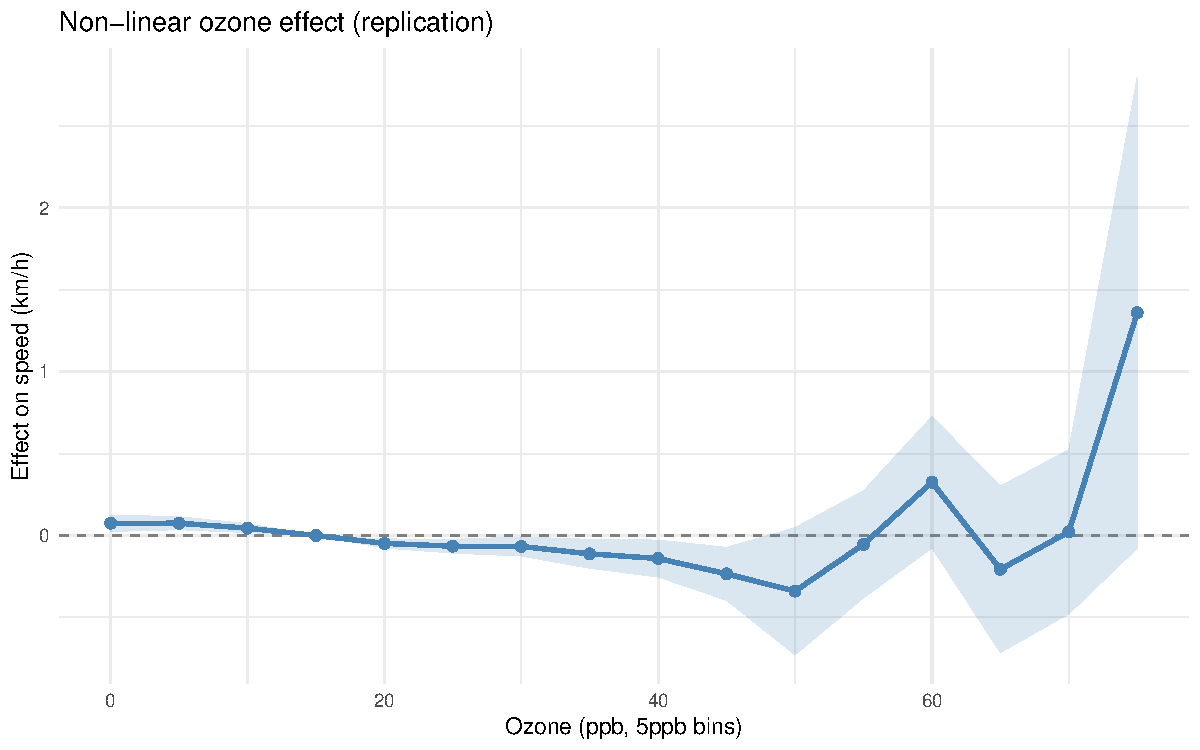
\includegraphics[width=\textwidth]{../output/figures/figure7_replication.pdf}
\caption{2013--2017}
\end{subfigure}
\hfill
\begin{subfigure}[b]{0.32\textwidth}
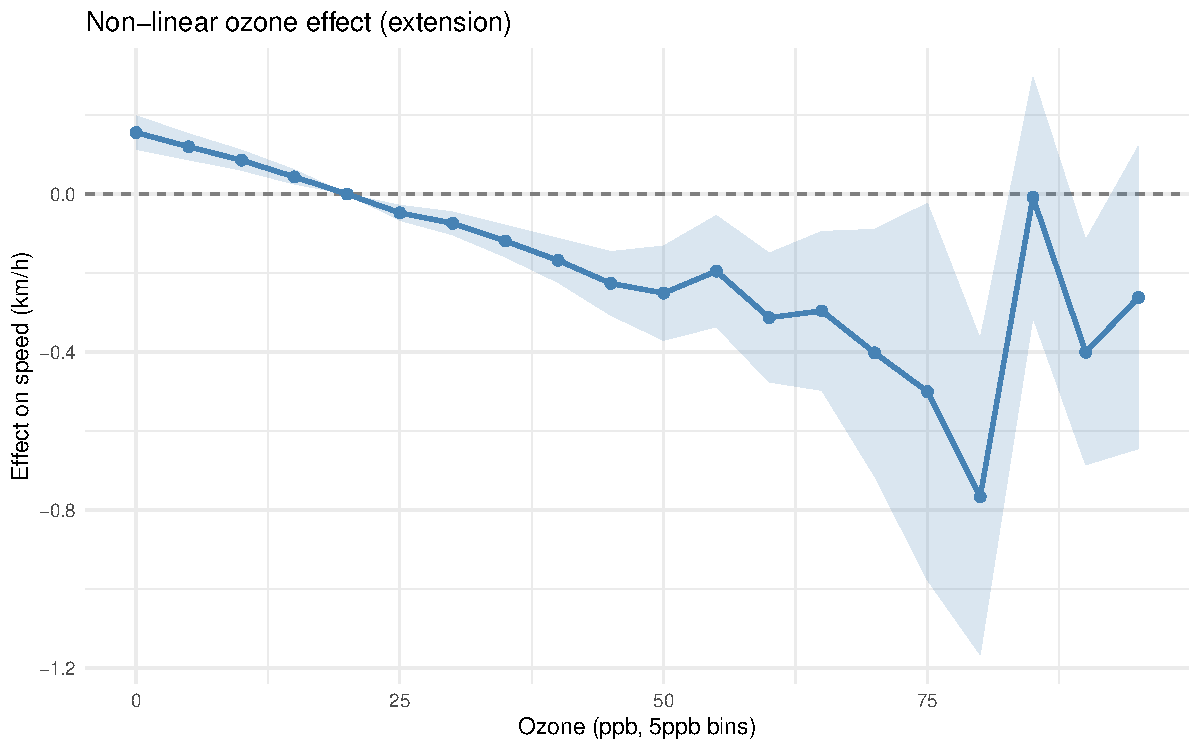
\includegraphics[width=\textwidth]{../output/figures/figure7_extension.pdf}
\caption{2013--2025}
\end{subfigure}
\hfill
\begin{subfigure}[b]{0.32\textwidth}
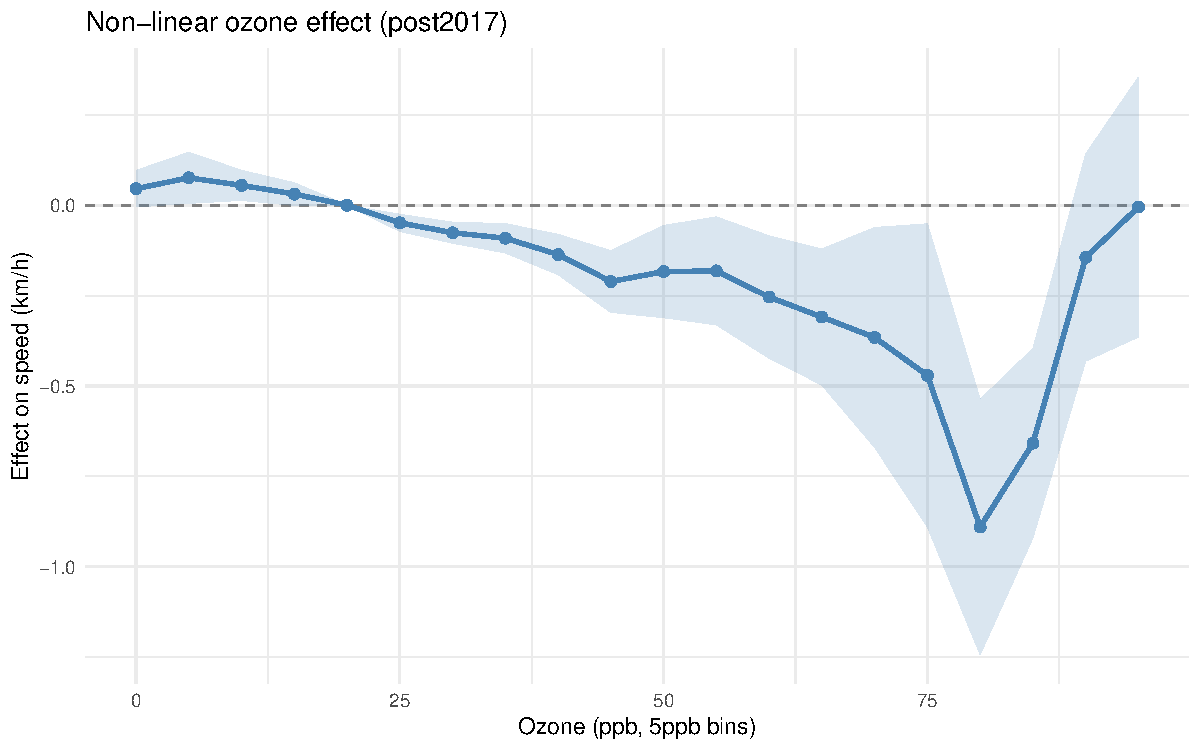
\includegraphics[width=\textwidth]{../output/figures/figure7_post2017.pdf}
\caption{2018--2025}
\end{subfigure}
\caption{Non-linear ozone effects (5~ppb dummies, within-day specification).}
\label{fig:nonlin}
\end{figure}

\paragraph{Lag and lead effects.} Figure~\ref{fig:lagslead} shows the lag/lead analysis. The contemporaneous effect is the strongest, with some persistence in the first lag reflecting ozone autocorrelation. Lead coefficients are near zero, supporting the causal interpretation.

\begin{figure}[H]
\centering
\begin{subfigure}[b]{0.32\textwidth}
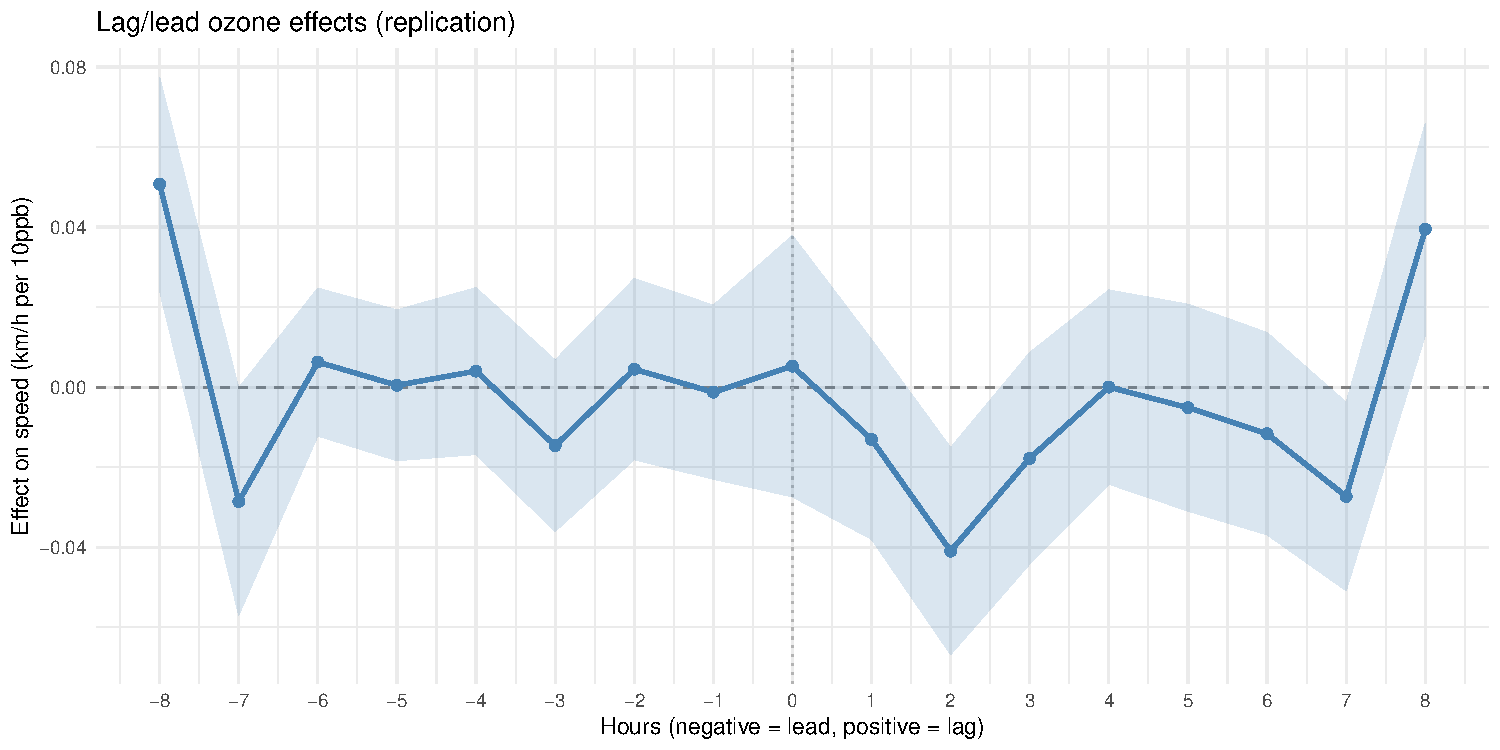
\includegraphics[width=\textwidth]{../output/figures/figure8_replication.pdf}
\caption{2013--2017}
\end{subfigure}
\hfill
\begin{subfigure}[b]{0.32\textwidth}
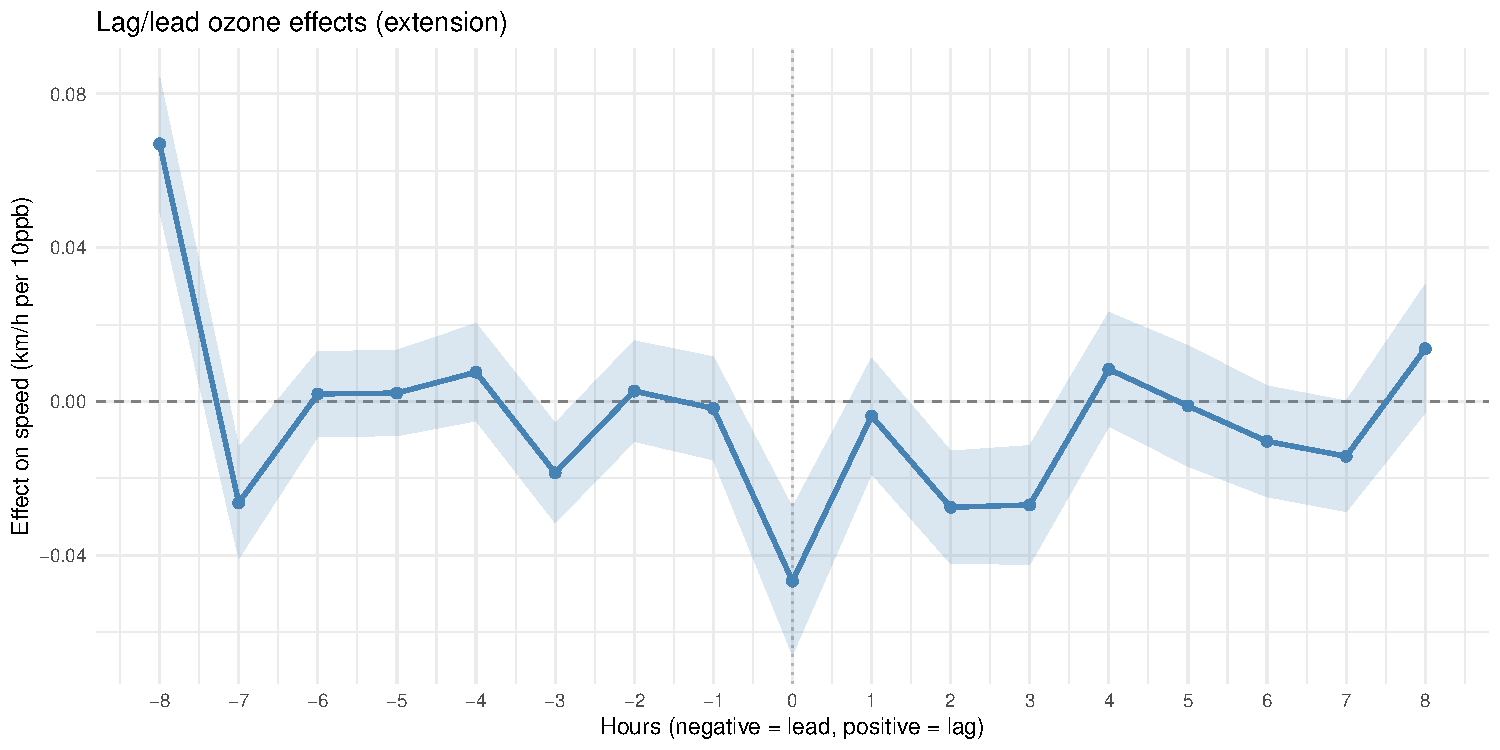
\includegraphics[width=\textwidth]{../output/figures/figure8_extension.pdf}
\caption{2013--2025}
\end{subfigure}
\hfill
\begin{subfigure}[b]{0.32\textwidth}
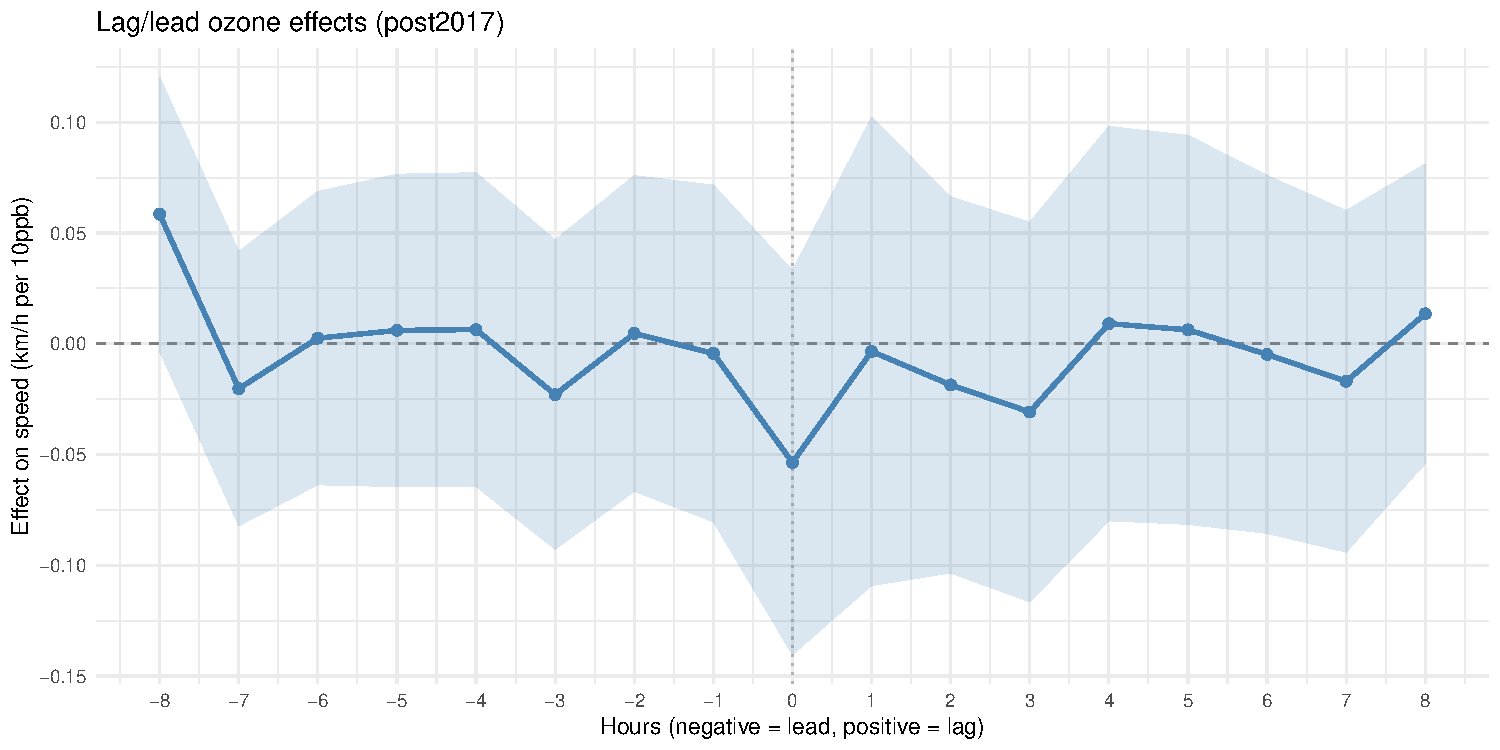
\includegraphics[width=\textwidth]{../output/figures/figure8_post2017.pdf}
\caption{2018--2025}
\end{subfigure}
\caption{Lag and lead ozone effects ($\pm$8 hours, within-day specification).}
\label{fig:lagslead}
\end{figure}

\paragraph{Median speed.} Using median rather than mean speed as the dependent variable yields within-day coefficients of $-0.040$ (replication), $-0.084$ (extension), and $-0.086$ (post-2017), confirming that outliers do not drive the results.


%% ============================================================
\section{Comparison with the Original Study} \label{sec:comparison}
%% ============================================================

Table~\ref{tab:comparison} summarizes the key ozone coefficients from \citet{klingen2020urban} alongside our replication and extension estimates. The coefficient represents the effect of a 10~ppb increase in ozone on cycling speed (km/h).

\begin{table}[H]
\centering
\caption{Comparison of ozone coefficients with \citet{klingen2020urban}.}
\label{tab:comparison}
\begin{tabular}{lcccc}
\toprule
Strategy & Original & Replication & Extension & Post-2017 \\
         & (2013--2017) & (2013--2017) & (2013--2025) & (2018--2025) \\
\midrule
Within-day        & $-0.053^{***}$ & $-0.052^{***}$ & $-0.095^{***}$ & $-0.098^{***}$ \\
Between-day       & $-0.083^{***}$ & $-0.286^{***}$ & $-0.125^{***}$ & $-0.084^{***}$ \\
Spatio-temporal (week) & $-0.044$  & $-0.029$       & $-0.071^{**}$  & $-0.089^{**}$  \\
Panel ($d \geq 0$) & $-0.026$ to $-0.031$ & $-0.024$ & $-0.026$ & $-0.020$ \\
\bottomrule
\end{tabular}

\medskip
\footnotesize Original estimates from \citet{klingen2020urban}: within-day from their Table~2 col.~1; between-day from Table~2 col.~2; spatio-temporal from Table~3 col.~2 (zone-week); panel range from Table~4. Our replication omits traffic controls; the original study showed these to be inconsequential. $^{***}$, $^{**}$: significant at 1\%, 5\%.
\end{table}

Several patterns emerge from the comparison. First, the within-day replication ($-0.052$) closely matches the original ($-0.053$), confirming that omitting traffic controls does not materially affect the estimate, as the original authors demonstrated. Second, the within-day effect is substantially larger in the post-2017 period ($-0.098$), which may reflect higher baseline ozone levels (25.4 vs.\ 18.9~ppb mean) and a shift in the cycling population toward more casual riders following infrastructure expansion. Third, our between-day replication ($-0.286$) exceeds the original ($-0.083$); this difference likely reflects different weather data sources (Open-Meteo vs.\ Met Office) and the absence of traffic controls, to which the between-day specification may be more sensitive. Fourth, the spatio-temporal estimates, while imprecise in the replication period, become significant in the extended and post-2017 samples as statistical power increases. Finally, the panel estimates are remarkably stable across all periods ($-0.020$ to $-0.026$), consistent with the original range, providing the strongest evidence that the ozone effect reflects within-cyclist physiological impairment.

%% ============================================================
\section{Conclusion} \label{sec:conclusion}
%% ============================================================

We replicate and extend \citet{klingen2020urban} using 108 million London bike-share trips spanning 2013--2025. The core finding---that ambient ozone reduces cycling speed at concentrations well below regulatory standards---holds robustly across all four identification strategies and all time periods examined. The within-day estimate nearly doubles in the post-2017 data, while the panel estimate remains stable, suggesting that the aggregate effect may partly reflect compositional changes in the cycling population alongside the underlying physiological mechanism.

The persistence of this effect through COVID-19, ULEZ expansion, and cycling infrastructure growth---and across a period in which NO$_x$ fell by half while ozone rose by a third---reinforces that it reflects a fundamental physiological response to ozone exposure rather than a statistical artifact of a particular period or pollution mix.

\newpage
\bibliography{references}

\end{document}
